\section*{Doble dioptra}

\item 
\begin{minipage}[t][3cm]{0.55\textwidth}
Una barra de material plástico transparente de la forma y dimensiones de la figura, es iluminada por una rendija.
Calcular la posición y tamaño de la imagen formada por cada una de las dioptras, y especificar si son reales o virtuales.
El índice de refracción es \num{1.56}.
Hacer un trazado de rayos a escala.
\end{minipage}
\begin{minipage}[c][0.4cm][t]{0.4\textwidth}
	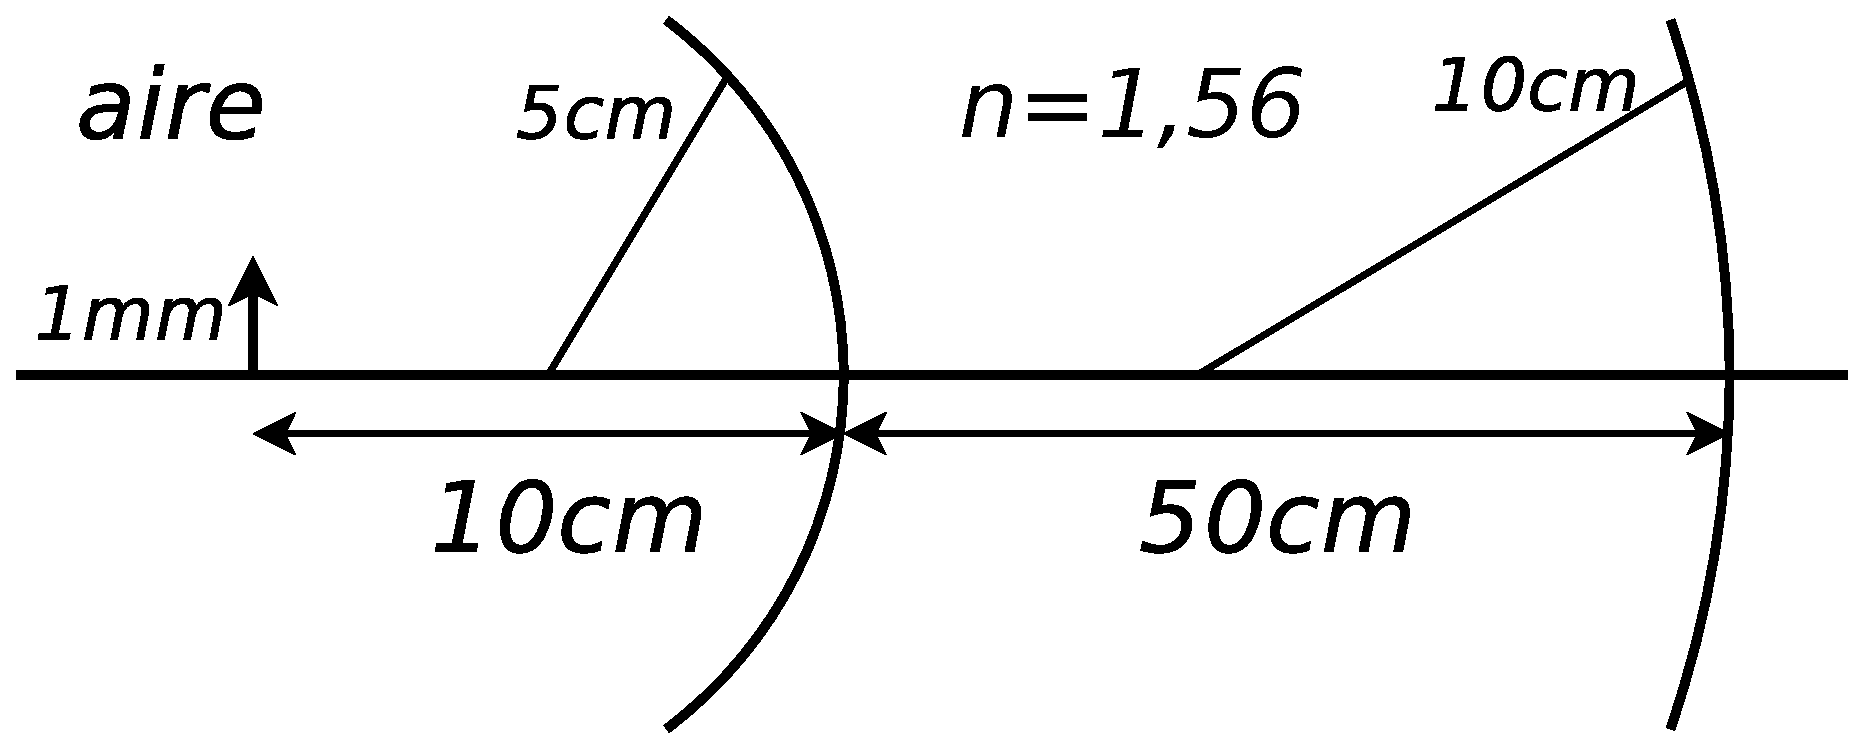
\includegraphics[width=\textwidth]{ej3-16}
\end{minipage}



\item
\begin{minipage}[t][1.5cm]{0.55\textwidth}
(*) La esfera de vidrio de la figura, de \SI{1}{\centi\metre} de diámetro, contiene una pequeña burbuja de aire desplazada \SI{0.5}{\centi\metre} de su centro.
Hallar la posición y el aumento de la burbuja cuando se la observa desde \emph{A} y desde \emph{B}.
\end{minipage}
\begin{minipage}[c][0.8cm][t]{0.4\textwidth}
	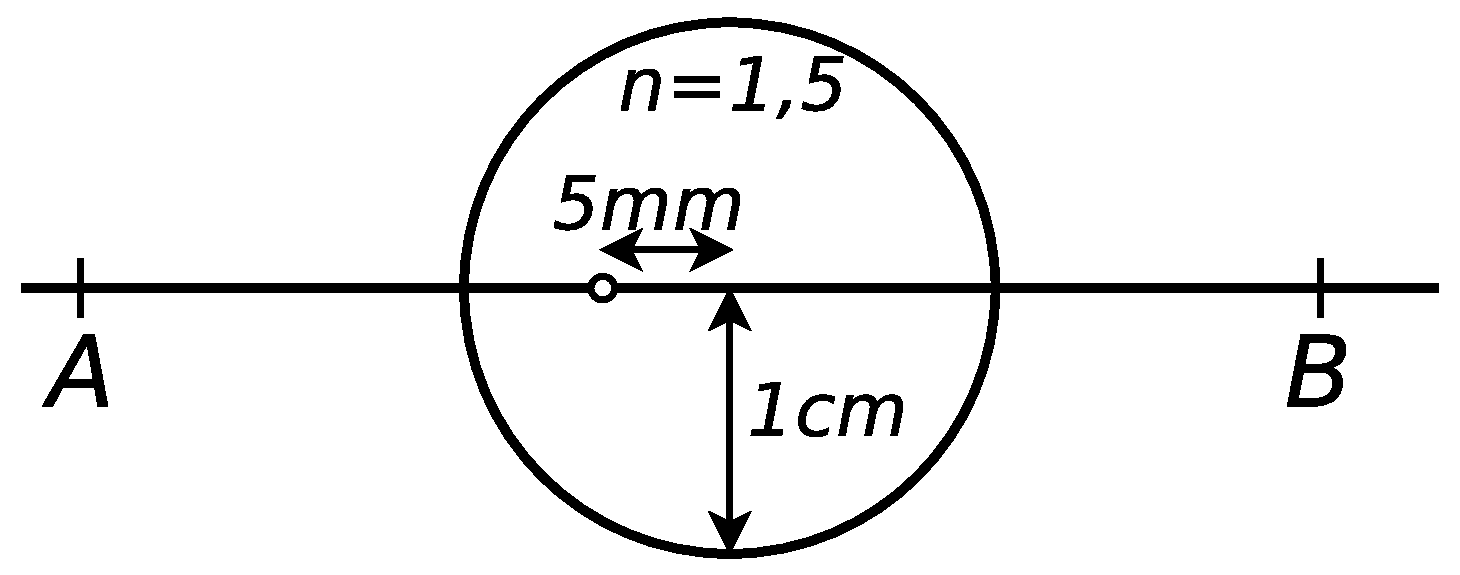
\includegraphics[width=\textwidth]{ej3-17}
\end{minipage}
